\chapter{Church-Turing Tese}

De maskiner vi har kigget på indtil videre har enten været med endelig hukommelse (Endelige Automater) eller med en uendelig hukommelse der kun fungerer i en LIFO stak-hukommelse. Dermed er de for begrænset til at kunne agere som modeller af generelt-formåls computere.

\section{Turingmaskiner}%
\label{sec:turingmachines}

I 1936 introducerede Alan Turing \textit{turingmaskinen}, en model som minder om en endelig automat, men med uendeligt og ubegrænset hukommelse. Denne model af en maskine kan alt det som en normal general purpose computer kan gøre. Dermed kan vi bruge denne model til at finde ud af begrænsninger m.m. om computere.

En turingmaskine bruger et uendeligt bånd som dets hukommelse. Den har en \textit{båndhoved} som kan læse \textit{og skrive} symboler og flytte sig selv rundt på båndet. Til at starte med indeholder båndet kan input strengen, dog kan den skrive på dette bånd. Til at læse informationen går båndhovedet over de symboler der skal læses. Maskinen bliver ved med at komputere indtil den vælger at producere et output, enten \textit{accept} eller \textit{afvis}. Hvis den ikke kommer til et accept eller afvis state, så kører den for evigt, uden nogensinde at stoppe.

\begin{figure}[ht]
  \centering
  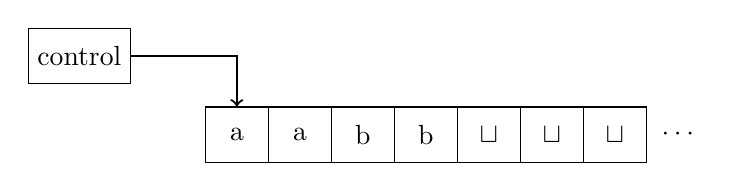
\begin{tikzpicture}
    \tikzset{block/.style={rectangle, draw, minimum height=2em, minimum width=3em}}
    \tikzset{line/.style={draw, -latex'}}
    \node[block] (control) {control};

    \node[block, minimum width=0.8cm] (a1) at (2,-1.0) {a};
    \node[block, minimum width=0.8cm] (a2) at (2.8,-1.0) {a};
    \node[block, minimum width=0.8cm] (b1) at (3.6,-1.0) {b};
    \node[block, minimum width=0.8cm] (b2) at (4.4,-1.0) {b};
    \node[block, minimum width=0.8cm] (b2) at (5.2,-1.0) {$\sqcup$};
    \node[block, minimum width=0.8cm] (b2) at (6.0,-1.0) {$\sqcup$};
    \node[block, minimum width=0.8cm] (b2) at (6.8,-1.0) {$\sqcup$};
    \node[label, minimum width=0.8cm] (b2) at (7.6,-1.0) {$\cdots$};

    \draw[->, thick] (control) -| (a1);
  \end{tikzpicture}
  \caption{\label{fig:turingschematic} Skematik af en turingmaskine.}
\end{figure}
I Figur~\ref{fig:turingschematic} kan der ses en skematik på en turingmaskine. Læg her mærke til at båndet er uendeligt langt, og efter input strengen er der bare blanke symboler, her betegnet som $\sqcup$.

Følgende punkter opsummerer forskellen mellem en endelig automat og en turingmaskine:

\begin{enumerate}
  \item En Turingmaskine kan både læse og skrive fra båndet.
  \item Læs-skriv (read-write) hovedet kan bevæge sig både til athøjre og til venstre.
  \item Båndet er uendeligt.
  \item De speceielle states til at acceptere og afvise et input træder i kraft med det samme.
\end{enumerate}

\subsection{Formel Definition af en Turingmaskine}%
\label{subsec:formaldefturingmachine}



Trods vi næsten aldrig bruger den formelle beskrivelse af en turingmaskine, da de oftest ender med at blive alt for store, giver vi den generelle formelle beskrivelse af en turingmaskine her.

Transitionsfunktionen i en turing maskine har formen $Q \times \Gamma \longrightarrow Q \times \Gamma \times \{L, R\}$. For eksempel betyder $\delta (q,a) = (r,b,L)$ at når båndet er over symbol $a$ og maskinen er i state $q$, så skal den skrive $b$ til symbolet hvor $a$ tidligere stod, og gå til state $r$. $L$ betyder her at den skal bevæge sig til venstre.

\begin{definition}[Formel Definition af en Turingmaskine]
  \label{def:formalturing}
  En \textbf{Turingmaskine} er en 7-tuple $(Q, \Sigma, \Gamma, \delta, q_{0}, q_{\text{accept}}, q_{\text{reject}})$, hvor $Q, \Sigma, \Gamma$ alle er endelige sæt, og
  \begin{enumerate}
    \item $Q$ er sættet af states.
    \item $\Sigma$ er inputalfabetet ikke indeholdende det blanke symbol, $\sqcup$.
    \item $\Gamma$ er båndalfabetet, hvor $\sqcup \in \Gamma$ og $\Sigma \subseteq \Gamma$.
    \item $\delta, Q \times \Gamma \longrightarrow Q \times \Gamma \times \{L, R\}$ er transitionsfunktionen.
    \item $q_{0} \in Q$ er startstaten.
    \item $q_{\text{accept}} \in Q$ er accept staten.
    \item $q_{\text{reject}} \in Q$ er afvis staten, hvor $q_{\text{accept}} \neq q_{\text{reject}}$.
  \end{enumerate}
\end{definition}

\subsection{Turingmaskine Komputering}%
\label{subsec:turingmaskinekomputering}

En turingmaskine komputere ved at starte sit båndhoved på den venstremest symbol på båndet. Inputtet $w = w_{1}w_{2} \ldots w_{n} \in \Sigma^{*}$ er på de første (venstremest) $n$ pladser på båndet, og det resterende er blankt. Siden $\Sigma$ ikke indeholder de blanke symbol, kan man være sikker på at så snart det blanke symbol kommer på båndet, har man læst inputtet færdigt. Hvis hovedet nogensinde forsøger at bevæge sig mere til venstre end muligt, så forbliver hovedet på den venstremest symbolplacering, trods den ``skal'' gå til venstre. Når $M$ er begyndt bevæger den sig efter reglerne beskrevet i transitionsfunktionen, indtil den enten accepterer eller afviser inputtet og dermed stopper. Hvis den hverken accepterer eller afviser inputtet kører den forevigt.

En \textit{konfiguration} er en kombination af de følgende tre ting:
\begin{itemize}
  \item Den nuværende state.
  \item Det nuværende indhold af båndet.
  \item Hovedet nuværende lokation.
\end{itemize}

De her konfigurationer bliver oftest repræsenteret på følgende måde: Givet en state $q$ og to strenge $u$ og $v$ over båndalfabetet $\Gamma$, skriver vi $uqv$ for konfigurationen hvor den nuværende state er $q$, båndindholdet er $uv$ og hovedets lokation er ved det andet symbol, altså $v$.

Vi siger at en kofngiruation $C_{1}$ \textit{giver} konfigurationen $C_{2}$ hvis turingmaskinen lovligt kan gå fra $C_{1}$ til $C_{2}$ på et enkelt skridt.

\textit{Startkonfigurationen} af $M$ på input $w$ er konfigurationen $q_{0}w$. Altså hvor staten er helt i start, og resterende af strengen, $w$ efterfølger. I en \textit{accepterende konfiguration} er staten i en konfiguration $q_{\text{accept}}$. I en \textit{afvisende konfiguration} er staten $q_{\text{reject}}$. Accept og afvisekonfigurationer er \textit{standsende konfigurationer}, altså konfigurationer som ikke giver flere konfigurationer.

Vi kalder samlingen af strenge som $M$ accepterer \textit{sproget af $M$} eller \textit{sproget genkendt af $M$}, betegnet $L(M)$.

\begin{definition}
Kald et sprog \textit{Turing-genkendeligt} hvis en Turingmaskine genkender det.
\end{definition}

Når en turingmaskine startes er tre resultater muligt, enten vil maskinen \textit{acceptere}, \textit{afvise} eller \textit{løkke}\footnote{\textit{loop} på engelsk}, hvor \textit{løkke} betyder at maskinen vil køre forevigt.

Vi kalder maskiner der aldrig kommer i en løkke for beslutningstagere\footnote{Måske? Deciders på engelsk.}, fordi de altid beslutter hvorvidt en streng skal accepteres eller afvises. En beslutningstager som genkender et sprog, siges også at \textit{beslutte} det sprog.

\begin{definition}
Kald et sprog Turing-besluttet eller simpelt besluttet, hvis en turingmaskine genkender det.
\end{definition}

%%% Local Variables:
%%% mode: latex
%%% TeX-engine: xetex
%%% TeX-command-extra-options: "-shell-escape"
%%% TeX-master: "main"
%%% End:
